\documentclass{beamer}
\usepackage[utf8]{inputenc}

% Use UTCS theme:
\usetheme[nousebiblatex]{utcs}

\usepackage[
backend=biber,
citestyle=authoryear,
style=authoryear,
hyperref=true
]{biblatex}
\usepackage{hyperref}
%Use utorange for hyperlinks
\hypersetup{colorlinks=true, allcolors=utblack, linkcolor=utblack,
  urlcolor=utorange, citecolor=utorange}

\usepackage[]{graphicx}
\usepackage[]{color}

\usepackage{accents}

\usepackage{subcaption}
\usepackage{tikz}
\usetikzlibrary{calc}
\usepackage[export]{adjustbox}
% externalize tikz
%\usetikzlibrary{external}
%\tikzexternalize[prefix=./tikz/]

\usepackage{amssymb,latexsym,amsmath}
\usepackage{amsfonts}
\usepackage{amsbsy}

\usepackage{minted}

\setbeamercovered{transparent}

\bibliography{presentation.bib}

\newcommand{\sep}{\setlength\arraycolsep{2pt}}
\def\disp{\displaystyle}

\author[BMS]{Robert Kirby$^{1}$
\and Andreas Kl\"ockner$^{2}$
\and Ben Sepanski$^{3}$
}
\date{25 March 2021}
\institute{$^{1}$Baylor University
\\ $^{2}$University of Illinois at Urbana-Champaign
\\ $^{3}$University of Texas at Austin
}
\title{Nonlocal UFL:\@ Finite elements for Helmholtz equations with a nonlocal boundary condition}
\logo{
\includegraphics[width=1.5cm]{figs/cslogo.eps}}

\begin{document}

%%%%%%%%%%%%%%%%%%%%%%%%             %%%%%%%%%%%%%%%%%%%%%%%%
%%%%%%%%%%%%%%%%%%%%%%%  Title frame  %%%%%%%%%%%%%%%%%%%%%%%%
%%%%%%%%%%%%%%%%%%%%%%%%             %%%%%%%%%%%%%%%%%%%%%%%%
\begin{frame}[noframenumbering]
    \titlepage
\end{frame}

%%%%%%%%%%%%%%%%%%%%%%%%     %%%%%%%%%%%%%%%%%%%%%%%%
%%%%%%%%%%%%%%%%%%%%%%%  TOC  %%%%%%%%%%%%%%%%%%%%%%%%
%%%%%%%%%%%%%%%%%%%%%%%%     %%%%%%%%%%%%%%%%%%%%%%%%
\begin{frame}[noframenumbering]{Order of Presentation}
    \tableofcontents
\end{frame}

\begin{frame}[noframenumbering]
\frametitle{Thanks to\ldots}
\begin{block}{}
\begin{itemize}
\item NSF 1525697, 1909176
\item The U.S. Department of Energy, Office of
Science, Office of Advanced Scientific Computing
Research, Department of Energy Computational Science
Graduate Fellowship under Award Number DE-SC0021110
\item Luke Olson (UIUC)
\end{itemize}
\end{block}
\end{frame}

%%%%%%%%%%%%%%%%%%%%%%%%                             %%%%%%%%%%%%%%%%%%%%%%%%
%%%%%%%%%%%%%%%%%%%%%%%  SECTION: Motivating problem  %%%%%%%%%%%%%%%%%%%%%%%%
%%%%%%%%%%%%%%%%%%%%%%%%                             %%%%%%%%%%%%%%%%%%%%%%%%
\section{Motivating Problem: Helmholtz scattering}

% slide numbers
\setbeamertemplate{footline}[frame number]

%%%%%%%%%%%%%%%%%%%%%%%%                             %%%%%%%%%%%%%%%%%%%%%%%%
%%%%%%%%%%%%%%%%%%%%%%%  Helmholtz radiation problem  %%%%%%%%%%%%%%%%%%%%%%%%
%%%%%%%%%%%%%%%%%%%%%%%%                             %%%%%%%%%%%%%%%%%%%%%%%%
\begin{frame}{Exterior scattering\footcite{Colton_Kress_1998,Kress_1999}}
    \begin{columns}
    \begin{column}{0.45\textwidth}
        \begin{figure}[ht]
        \begin{center}
        \begin{tikzpicture}[scale=0.8]
            \draw [thick,fill=black!30] (-3,-3) rectangle (3,3)
            (0, 0) circle (1);
            \node at (0,0) {$\Omega^c$};
            \node at (-2,2) {$\Omega'$};
            \node [anchor=west] at (1,0) {$\Gamma$};
            \node [anchor=west] at (3,0) {$\Sigma$};
        \end{tikzpicture}
        \end{center}\label{fig:2ddomain}
        \end{figure}
    \end{column}
    \begin{column}{0.55\textwidth}
        \begin{itemize}
            \item<1-> Model waves reflecting off of obstacle $\Gamma$
            \[
                \begin{cases}
                    -\Delta u - \kappa^2 u = 0, &  \mathbb R^d\setminus\Omega^c \\
                    \frac{\partial u}{\partial n} = f, & \Gamma
                \end{cases}
            \]
            \item<2-> \emph{Without} any spurious reflections from infinity
            \[
                \lim_{r\to\infty} r^{(d-1)/2}
                    \left(\tfrac{\partial u}{\partial r} - i\kappa u\right)
                = 0
            \]
            \item<3-> In some finite domain of interest 
            $\Omega'\subseteq \mathbb R^d\setminus\Omega^c$
            bounded by $\Sigma$.
        \end{itemize}
    \end{column}
\end{columns}
\end{frame}

%%%%%%%%%%%%%%%%%%%%%%%%                   %%%%%%%%%%%%%%%%%%%%%%%%
%%%%%%%%%%%%%%%%%%%%%%%  But what are BCs?  %%%%%%%%%%%%%%%%%%%%%%%%
%%%%%%%%%%%%%%%%%%%%%%%%                   %%%%%%%%%%%%%%%%%%%%%%%%
\begin{frame}{Exterior scattering: computational problem}
    \begin{columns}
    \begin{column}{0.45\textwidth}
        \begin{figure}[ht]
        \begin{center}
        \begin{tikzpicture}[scale=0.8]
            \draw [thick,fill=black!30] (-3,-3) rectangle (3,3)
            (0, 0) circle (1);
            \node at (0,0) {$\Omega^c$};
            \node at (-2,2) {$\Omega'$};
            \node [anchor=west] at (1,0) {$\Gamma$};
            \node [anchor=west] at (3,0) {$\Sigma$};
        \end{tikzpicture}
        \end{center}
        \end{figure}
    \end{column}
    \begin{column}{0.55\textwidth}
        \begin{itemize}
            \item<1-> Problem we want to solve
            \[
                \begin{cases}
                    -\Delta u - \kappa^2 u = 0, &  \mathbb R^d\setminus\Omega \\
                    \frac{\partial u}{\partial n} = f, & \Gamma \\
                    \lim_{r\to\infty} r^{(d-1)/2}
                        \left(\tfrac{\partial u}{\partial r} - i\kappa u\right)
                = 0
                \end{cases}
            \]
            \item<2-> Problem we can actually solve
            \[
                \begin{cases}
                    -\Delta u - \kappa^2 u = 0, & \Omega' \\
                    \frac{\partial u}{\partial n} = f, & \Gamma \\
                    ?????, & \Sigma
                \end{cases}
            \]
        \end{itemize}
    \end{column}
    \end{columns}
\end{frame}


%%%%%%%%%%%%%%%%%%%%%%%%              %%%%%%%%%%%%%%%%%%%%%%%%
%%%%%%%%%%%%%%%%%%%%%%%  PML Approach  %%%%%%%%%%%%%%%%%%%%%%%%
%%%%%%%%%%%%%%%%%%%%%%%%              %%%%%%%%%%%%%%%%%%%%%%%%
\begin{frame}{Exterior scattering: Perfectly Matched Layers (PML)\footcite{BERENGER1994185,Erlangga_2006,Bermudez_Hervella-Nieto_Prieto_Rodrguez_2006}}
    \begin{columns}
    \begin{column}{0.45\textwidth}
        \begin{figure}[ht]
        \begin{center}
         \begin{tikzpicture}[scale=0.6]
            \draw [thick,fill=black!60] (-4,-4) rectangle (4,4);
            \draw [thick,fill=black!30] (-3,-3) rectangle (3,3);
            \draw [fill=white] (0, 0) circle (1);
          \node at (0,0) {$\Omega^c$};
          \node at (-2,2) {$\Omega'$};
          \node [anchor=west] at (1,0) {$\Gamma$};
          \node [anchor=west] at (3,0) {$\Omega_S$};
          \node [anchor=west] at (4,0) {$\Sigma$};
        \end{tikzpicture}
        \end{center}
        \end{figure}
        \vfill
    \end{column}
    \begin{column}{0.55\textwidth}
        \[
            \begin{cases}
                -\nabla \cdot \beta(x) \nabla u - \kappa^2 u = 0,  & \Omega^\prime \\
                \frac{\partial u}{\partial n}  =  f, &\Gamma \\
                u = 0, &\Sigma
            \end{cases}
        \]
            \begin{itemize}
              \item<2-> $\Omega'$: $\beta = I$, satisfies original equation
              \item<3-> $\Omega_S$: $\beta$ is a complex-valued coordinate transform to cause exponential decay
              in oscillating waves
              \item<4-> {\bf Preconditioning is difficult!\footnotemark}
            \end{itemize}
    \end{column}
    \end{columns}
    \footcitetext{EngquistPMLPreconditioner2011,Safin_Minkoff_Zweck_2018}
\end{frame}

%%%%%%%%%%%%%%%%%%%%%%%%                           %%%%%%%%%%%%%%%%%%%%%%%%
%%%%%%%%%%%%%%%%%%%%%%%  Integral equations review  %%%%%%%%%%%%%%%%%%%%%%%%
%%%%%%%%%%%%%%%%%%%%%%%%                           %%%%%%%%%%%%%%%%%%%%%%%%
\section{A nonlocal boundary condition}

\begin{frame}{Integral form of the solution}
    \begin{columns}
      \begin{column}{0.7\textwidth}
             Using the Helmholtz Green's function \[\mathcal K\left(\mathbf{x}\right)
                =\displaystyle\frac{i}{4\pi \left|\mathbf{x}\right|}
                \displaystyle e^{i\kappa\left|\mathbf{x}\right|},\]
      \end{column}
      \begin{column}{0.3\textwidth}
        \begin{figure}
        \begin{center}
          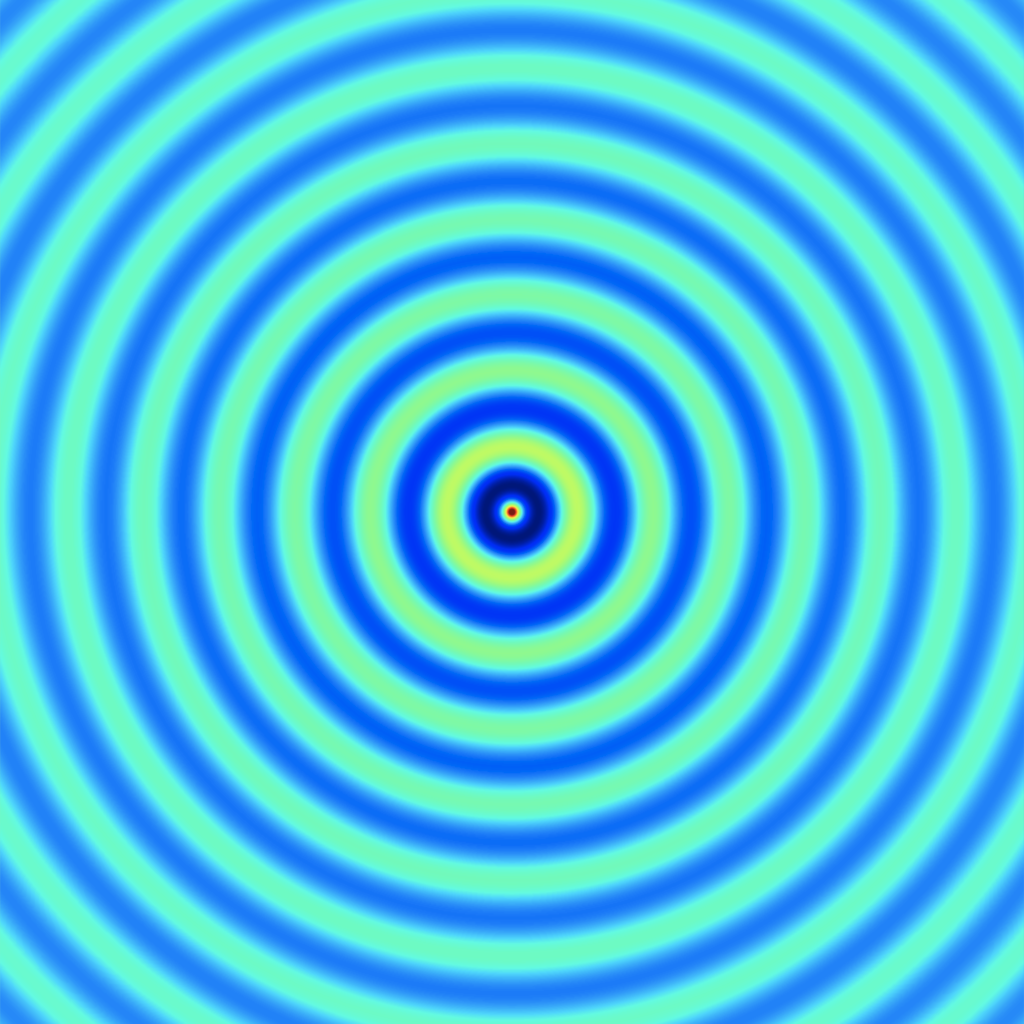
\includegraphics[width=0.5\textwidth]{images/2d_helmholtz_greens_function.png}
          \end{center}\caption{$\mathcal K$ in 2D}
          \end{figure}
      \end{column}
    \end{columns}

    \uncover<2->{
    the \emph{true solution} satisfies          \footcite{Colton_Kress_1998,Kress_1999}

      \begin{equation*}
          u(x) = D(u)(x) - S(\tfrac{\partial u}{\partial n})(x), \quad x \in\Omega'
      \end{equation*}
      where
      }
    \uncover<3->{
        \begin{align*}
            D(u)(x) &= \int_\Gamma \left( \tfrac{\partial}{\partial n} \mathcal K( x-y) \right)u(y) \,dy, 
            \\
            S(u)(x) &= \int_\Gamma \mathcal K (x - y ) u(y)\,dy
        \end{align*}
    }
\end{frame}

%%%%%%%%%%%%%%%%%%%%%%%        %%%%%%%%%%%%%%%%%%%%%%%%
%%%%%%%%%%%%%%%%%%%%%%  Our BC  %%%%%%%%%%%%%%%%%%%%%%%%
%%%%%%%%%%%%%%%%%%%%%%%        %%%%%%%%%%%%%%%%%%%%%%%%
\begin{frame}{Exterior scattering}
  \begin{columns}
    \begin{column}{0.35\textwidth}
    \begin{figure}[ht]
        \begin{center}
        \begin{tikzpicture}[scale=0.4]
          \draw [thick,fill=black!30] (-3,-3) rectangle (3,3)
            (0, 0) circle (1);
          \node at (0,0) {$\Omega^c$};
          \node at (-2,2) {$\Omega'$};
          \node [anchor=west] at (1,0) {$\Gamma$};
          \node [anchor=west] at (3,0) {$\Sigma$};
        \end{tikzpicture}
        \end{center}
        %\caption{A 2D example of a truncated domain}
        %\label{fig:2ddomain}
      \end{figure}
        \end{column}
        \begin{column}{0.65\textwidth}
                \emph{Exact} boundary conditions
                 \[
                     \begin{cases}
                         -\Delta u - \kappa^2 u = 0, & \Omega' \\
                         \frac{\partial u}{\partial n} = f, & \Gamma \\
                         (i \kappa- \tfrac{\partial}{\partial n})\left( u - D(u) + S(f) \right) = 0, & \Sigma
                     \end{cases}
                 \]
        \end{column}
    \end{columns}

    \uncover<2->{
    \hfill
    \begin{block}{Variational Form:}
        For all $v\in H^1(\Omega')$
        \vspace{1mm}
        \begin{alignat*}{2}
            \left( \nabla u, \nabla v \right)
            - \kappa^2 \left( u, v \right)
            - i\kappa &\langle u, v \rangle_\Sigma
            &+ \langle \left(i\kappa - \tfrac{\partial}{\partial n}\right)D(u), v \rangle_\Sigma
            \\
            = \;&\langle f, v \rangle_\Gamma
                &+ \langle \left(i\kappa - \tfrac{\partial}{\partial n}\right)
                    S(f), v \rangle_\Sigma
        \end{alignat*}
        \vspace{1mm}
    \end{block}
    }
\end{frame}


%%%%%%%%%%%%%%%%%%%%%%%%                     %%%%%%%%%%%%%%%%%%%%%%%%
%%%%%%%%%%%%%%%%%%%%%%%  Theoretical results  %%%%%%%%%%%%%%%%%%%%%%%%
%%%%%%%%%%%%%%%%%%%%%%%%                     %%%%%%%%%%%%%%%%%%%%%%%%
\begin{frame}{Theory}
    \begin{itemize}
        \item<2-> $a$ is a bounded bilinear form on $H^1 \times H^1$
        \item<3-> $F$ is a bounded linear functional on $H^1$
        \item<4-> G{\aa}rding inequality. There exist $M$ and an $\alpha > 0$ such that
        \begin{equation*}
            \operatorname{Re}(a(u,u)) + M \left\| u \right\|^2 \geq \alpha \left\| u \right\|_{H^1(\Omega)}^2.
            \end{equation*}
        \item<5-> For $h \leq h_0$, we have optimal-order $H^1$ and $L^2$ error estimates.\footcite{kirby2021finite}
    \end{itemize}
\end{frame}

%%%%%%%%%%%%%%%%%%%%%%%%                       %%%%%%%%%%%%%%%%%%%%%%%%
%%%%%%%%%%%%%%%%%%%%%%%  SECTION: Nonlocal UFL  %%%%%%%%%%%%%%%%%%%%%%%%
%%%%%%%%%%%%%%%%%%%%%%%%                       %%%%%%%%%%%%%%%%%%%%%%%%
\section{Nonlocal UFL}

%%%%%%%%%%%%%%%%%%%%%%%%              %%%%%%%%%%%%%%%%%%%%%%%%
%%%%%%%%%%%%%%%%%%%%%%%  Requirements  %%%%%%%%%%%%%%%%%%%%%%%%
%%%%%%%%%%%%%%%%%%%%%%%%              %%%%%%%%%%%%%%%%%%%%%%%%
\begin{frame}{Nonlocal operations in UFL}
    \begin{itemize}
        \item \emph{Recall:} 
        \only<-5>{
            \[
                D(u)(x) = \int_{\Gamma} \tfrac{\partial}{\partial n}\mathcal K(x - y) u(y) \,dy,
                \qquad x\in \Sigma
            \]
        }
        \only<6->{
            \[
                D(u)({\color{utorange}x}) = 
                \int_{\color{blue}\Gamma} 
                \tfrac{\partial}{\partial n}\mathcal K({\color{utorange}x} - 
                {\color{blue}y}) u({\color{blue}y})
                \,d{\color{blue}y},
                \qquad {\color{utorange}x}\in{\color{utorange}\Sigma}
            \]
        }
        \item<2-> \emph{Problem:} Nonlocal operations have large support (all of
            $\Sigma$!)
        \begin{itemize}
            \item<3-> This makes our stiffness matrix dense, especially
                in 3D
            \item<4-> \emph{Solution:} Firedrake's matrix-free evaluation
        \end{itemize}
        \vfill
        \item<5-> \emph{Problem:} Naive evaluation of layer potentials is slow:
        \begin{itemize}
            \item<7-> $\operatorname{ndof}(\Gamma)\cdot \operatorname{ndof}(\Sigma)$
            \item<8-> \emph{Solution:} Fast multipole methods (FMM)\footcite{Carrier_Greengard_Rokhlin_1988}: use the structure of $\mathcal K$ to compute the potential in \emph{linear time} with low-rank approximations
        \end{itemize}
    \end{itemize}
\end{frame}

%%%%%%%%%%%%%%%%%%%%%%%%                       %%%%%%%%%%%%%%%%%%%%%%%%
%%%%%%%%%%%%%%%%%%%%%%%  Building BEM into UFL  %%%%%%%%%%%%%%%%%%%%%%%%
%%%%%%%%%%%%%%%%%%%%%%%%                       %%%%%%%%%%%%%%%%%%%%%%%%
\begin{frame}{Nonlocal operations in UFL:\@ Marshalling pytential\footcite{KlöcknerPytential}}
    \begin{itemize}
        \item Build \mintinline{python}{LayerPotential} as a UFL External Operator\footnote{N. Bouziani, \emph{External Operators}:
        {\tiny\url{https://fenics2021.com/talks/bouziani.html}}}
            \begin{itemize}
                \vfill
                \item<2->[\checkmark] Build pytential representation
                    of domain of interest
                \only<3>{
                    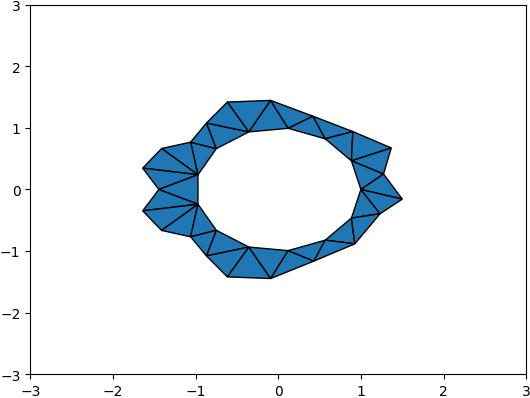
\includegraphics[width=0.65\textwidth]{images/coarse_near_gamma2d.png}
                }
                \only<-2,4->{
                    \vfill
                    \item<4->[\checkmark] Build pytential representation
                        of function space
                    \vfill
                    \item<5->[\checkmark] Build efficient converter between
                        pytential and firedrake representations
                    \vfill
                    \item<6-> Fully support automatic differentiation
                }
            \end{itemize}
        \vfill
        \only<-2,4->{
        \item<7-> Evaluation of $\left\langle(i\kappa - \tfrac{\partial}{\partial n})D(u), v\right\rangle_\Sigma$ 
            \begin{itemize}
                \vfill
                \item<8->[\checkmark] \mintinline{python}{LayerPotential} evaluates $D(u)$ (automatically uses pytential, which employs FMM to compute the potential)
                \vfill
                \item<9->[\checkmark] Firedrake evaluates inner product
            \end{itemize}
        }
        \end{itemize}
\end{frame}

%%%%%%%%%%%%%%%%%%%%%%%%                                    %%%%%%%%%%%%%%%%%%%%%%%
%%%%%%%%%%%%%%%%%%%%%%%  Express our problem with firedrake  %%%%%%%%%%%%%%%%%%%%%%%
%%%%%%%%%%%%%%%%%%%%%%%%                                    %%%%%%%%%%%%%%%%%%%%%%%
\begin{frame}[fragile]{Solving the system with Firedrake}
    Extend UFL:
    \[
        a(u, v)
        = \left( \nabla u , \nabla v \right) - \kappa^2 \left( u , v \right)
        - i \kappa \langle u, v \rangle_{\Sigma}
        + \langle \left( i \kappa - \tfrac{\partial}{\partial n} \right) D(u)  v \rangle_\Sigma
    \]
    \visible<2->{
    Will be written as:
    \begin{figure}[ht]
        \begin{center}
            \only<-2>{
            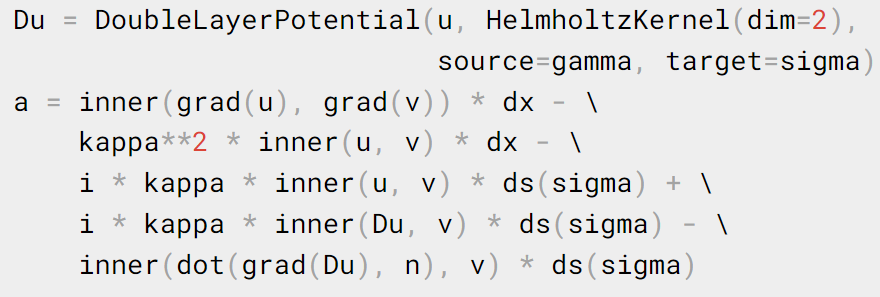
\includegraphics[width=\textwidth]{images/code.png}
            }
            \only<3->{
            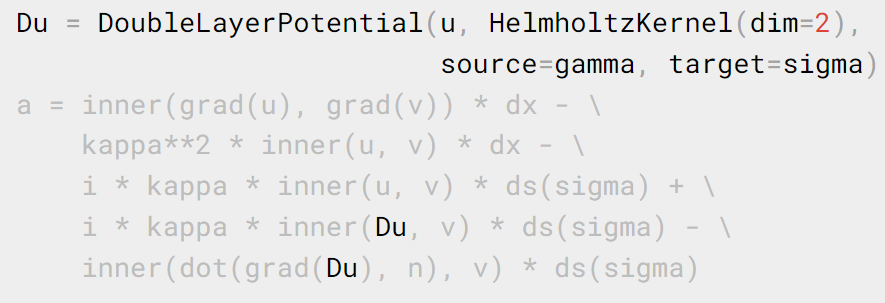
\includegraphics[width=\textwidth]{images/code-focused.png}
            }
        \end{center}
    \end{figure}
    }
\end{frame}

\section{Numerical Results}

%%%%%%%%%%%%%%%%%%%%%%%%                %%%%%%%%%%%%%%%%%%%%%%%%
%%%%%%%%%%%%%%%%%%%%%%%  Accuracy plots  %%%%%%%%%%%%%%%%%%%%%%%%
%%%%%%%%%%%%%%%%%%%%%%%%                %%%%%%%%%%%%%%%%%%%%%%%%
\begin{frame}{Numerical results: 2D}
    \begin{figure}[ht]
    \begin{center}
        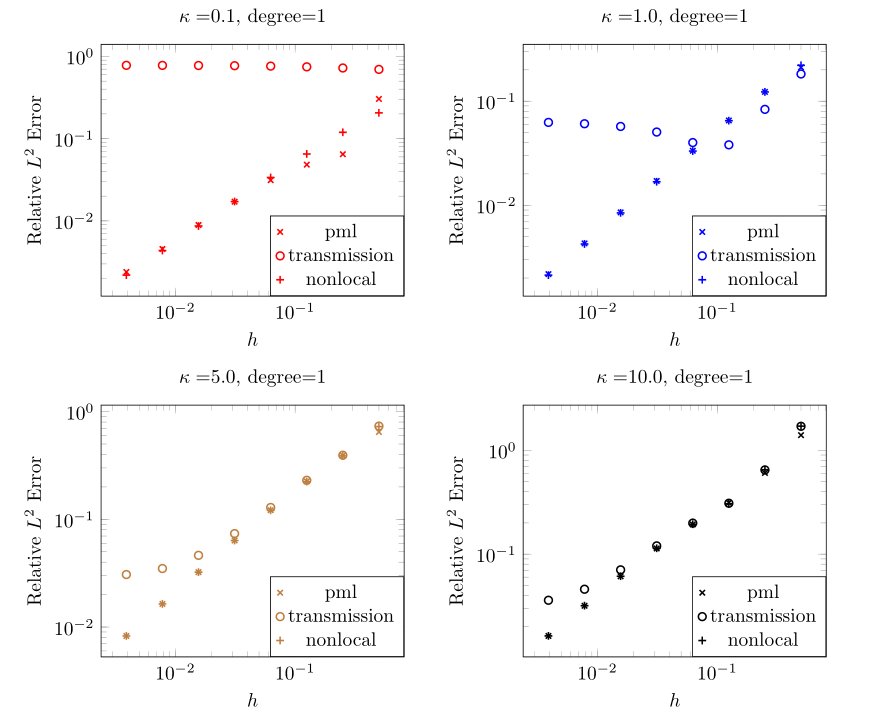
\includegraphics[width=0.8\textwidth]{images/degree-1-accuracy.png}
    \end{center}
    \end{figure}
\end{frame}

%%%%%%%%%%%%%%%%%%%%%%%%                 %%%%%%%%%%%%%%%%%%%%%%%%
%%%%%%%%%%%%%%%%%%%%%%%  Preconditioning  %%%%%%%%%%%%%%%%%%%%%%%%
%%%%%%%%%%%%%%%%%%%%%%%%                 %%%%%%%%%%%%%%%%%%%%%%%%
\begin{frame}{Preconditioning: LU of local part}
    \begin{figure}[ht]
    \begin{center}
        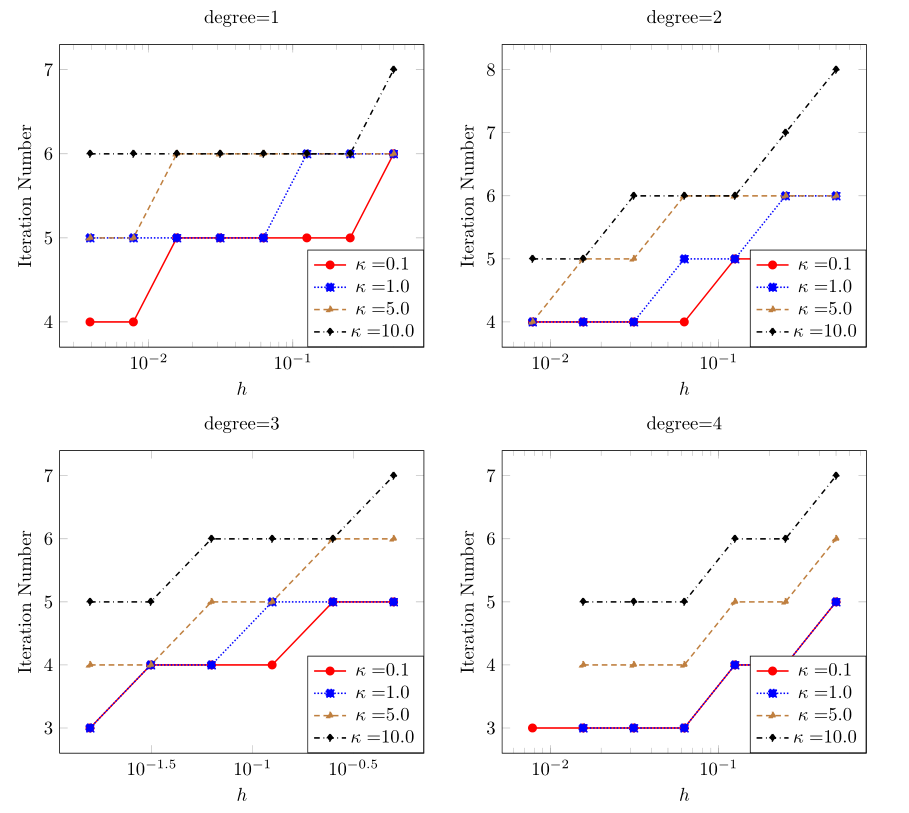
\includegraphics[width=0.75\textwidth]{images/iteration-pc-by-transmission.png}
    \end{center}
    \end{figure}
\end{frame}

%%%%%%%%%%%%%%%%%%%%%%%%       %%%%%%%%%%%%%%%%%%%%%%%%
%%%%%%%%%%%%%%%%%%%%%%%  pyamg  %%%%%%%%%%%%%%%%%%%%%%%%
%%%%%%%%%%%%%%%%%%%%%%%%       %%%%%%%%%%%%%%%%%%%%%%%%
\begin{frame}{Preconditioning: PyAMG}
    \begin{itemize}
        \item If we can find a good preconditioner for the local
            problem, we get a good preconditioner for the nonlocal
            problem
        \vfill
        \item<2->PyAMG:\@ precondition with plane waves
            \begin{figure}[ht]
            \begin{center}
                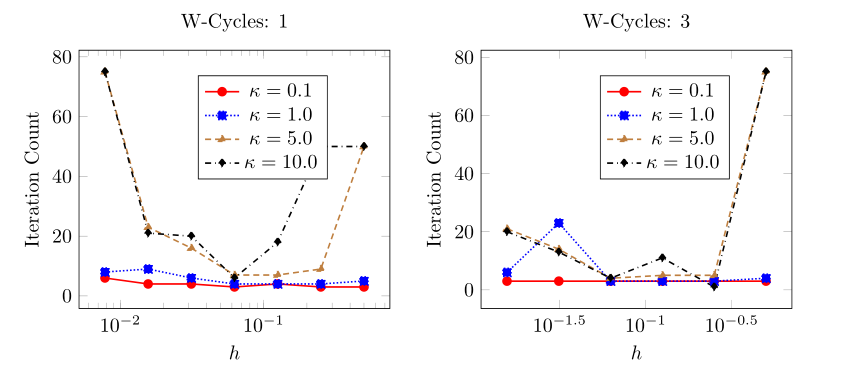
\includegraphics[width=0.8\textwidth]{images/pyamg.png}
            \end{center}
            \end{figure}
    \end{itemize}
\end{frame}

%%%%%%%%%%%%%%%%%%%%%%%%             %%%%%%%%%%%%%%%%%%%%%%%%
%%%%%%%%%%%%%%%%%%%%%%%  Conclusion  %%%%%%%%%%%%%%%%%%%%%%%%
%%%%%%%%%%%%%%%%%%%%%%%%             %%%%%%%%%%%%%%%%%%%%%%%%
\begin{frame}{Conclusion}
    \begin{columns}
        \begin{column}{0.55\textwidth}
        \begin{block}{Results}
            \begin{itemize}
                \item Novel nonlocal boundary condition
                \begin{itemize}
                    \item Error estimates
                    \footnotemark
                \end{itemize}
                \item Extension of UFL to efficiently handle nonlocal operators
                \item Numerical experiments demonstrating optimal-order convergence
                \item Investigation into preconditioners
            \end{itemize}
        \end{block}
        \end{column}
        \begin{column}{0.45\textwidth}
        \begin{block}{Coming Soon}
            \begin{itemize}
                \item Full implementation of \mintinline{python}{LayerPotential}s
                and \mintinline{python}{VolumePotential}\footnotemark s in UFL as External Operator\footnotemark s
                
                \item General theory for this method and application to more problems
            \end{itemize}
        \end{block}
        \end{column}
    \end{columns}
    \vfill
    % have to handle footnote counting manually
    \addtocounter{footnote}{-1}
    \footcitetext{kirby2021finite}
    \stepcounter{footnote}
    \footnotetext{X. Wei, \emph{IEM-FEM Coupling}:
        {\tiny\url{https://fenics2021.com/talks/wei.html}}}
    \stepcounter{footnote}
     \footnotetext{N. Bouziani, \emph{External Operators}:
        {\tiny\url{https://fenics2021.com/talks/bouziani.html}}}
\end{frame}

\begin{frame}[noframenumbering,allowframebreaks]{References}
    \printbibliography
\end{frame}

%%%%%%%%%%%%%%%%%%%%%%%%               %%%%%%%%%%%%%%%%%%%%%%%%
%%%%%%%%%%%%%%%%%%%%%%%  Backup slides  %%%%%%%%%%%%%%%%%%%%%%%%
%%%%%%%%%%%%%%%%%%%%%%%%               %%%%%%%%%%%%%%%%%%%%%%%%
\begin{frame}[noframenumbering]
    \begin{center}
        Backup Slides
    \end{center}
\end{frame}

%%%%%%%%%%%%%%%%%%%%%%%%                      %%%%%%%%%%%%%%%%%%%%%%%%
%%%%%%%%%%%%%%%%%%%%%%%  Extra accuracy plots  %%%%%%%%%%%%%%%%%%%%%%%%
%%%%%%%%%%%%%%%%%%%%%%%%                      %%%%%%%%%%%%%%%%%%%%%%%%
\begin{frame}[noframenumbering]{Numerical results: 2D, degree 2}
    \begin{figure}[ht]
    \begin{center}
        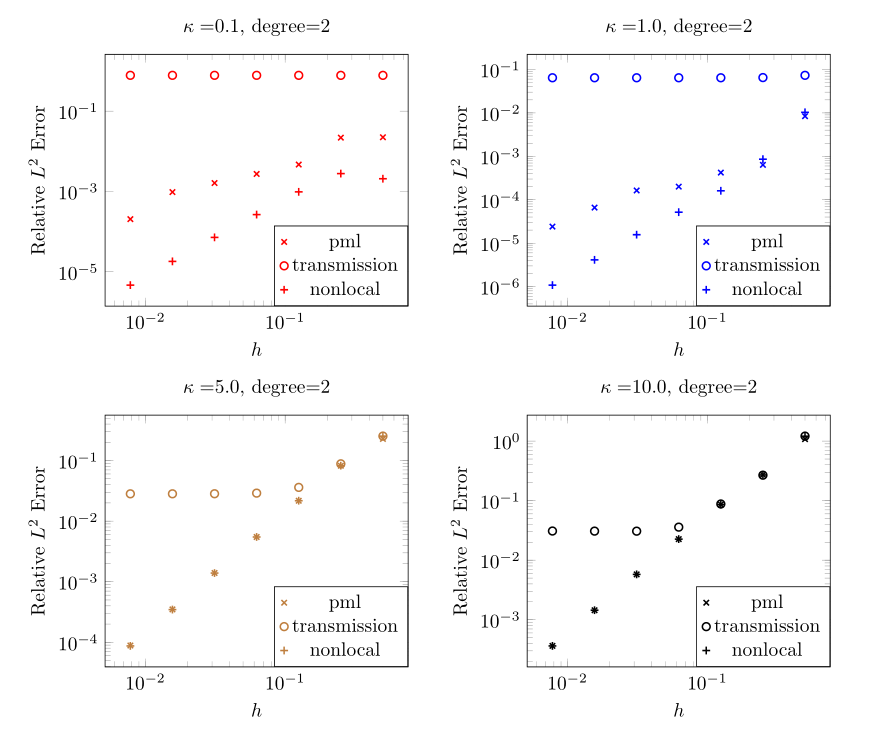
\includegraphics[width=0.8\textwidth]{images/degree-2-accuracy.png}
    \end{center}
    \end{figure}
\end{frame}
\begin{frame}[noframenumbering]{Numerical results: 2D, degree 3}
    \begin{figure}[ht]
    \begin{center}
        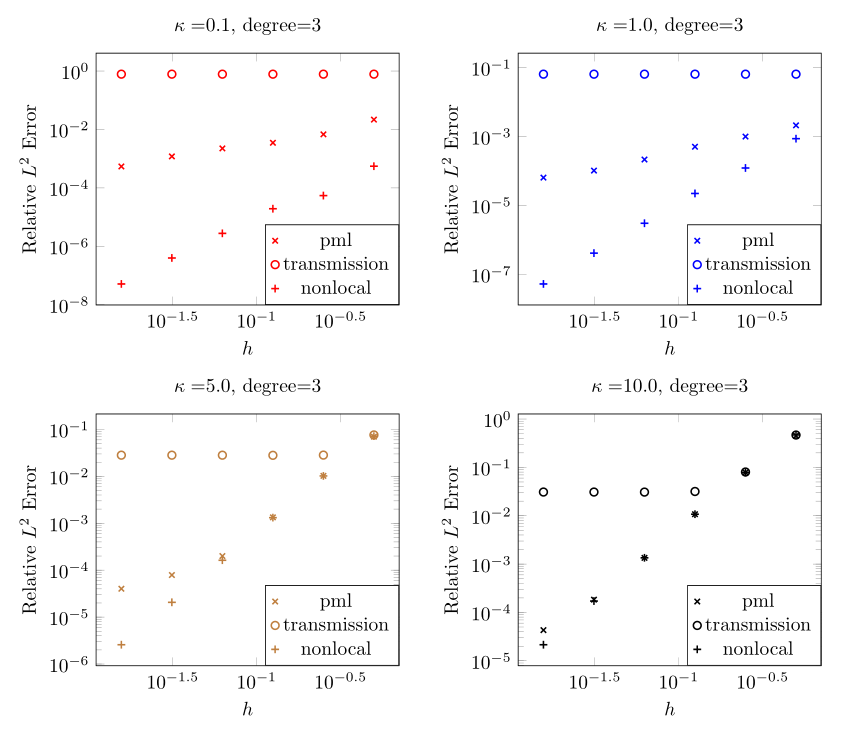
\includegraphics[width=0.8\textwidth]{images/degree-3-accuracy.png}
    \end{center}
    \end{figure}
\end{frame}
\begin{frame}[noframenumbering]{Numerical results: 2D, degree 4}
    \begin{figure}[ht]
    \begin{center}
        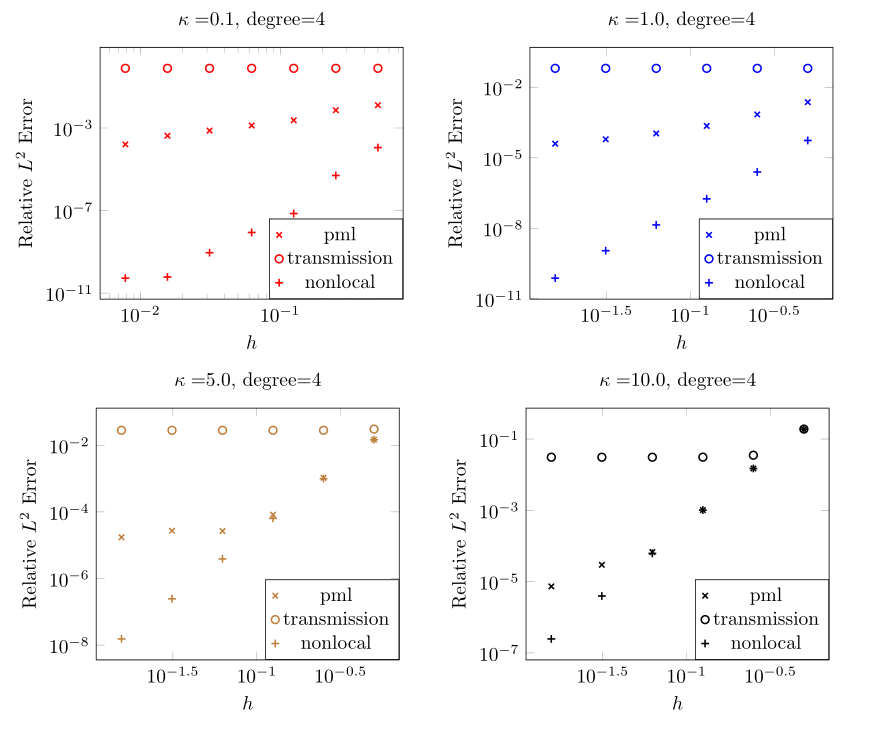
\includegraphics[width=0.8\textwidth]{images/degree-4-accuracy.png}
    \end{center}
    \end{figure}
\end{frame}
\begin{frame}[noframenumbering]{Numerical results: 3D, degree 1}
    \begin{figure}[ht]
    \begin{center}
        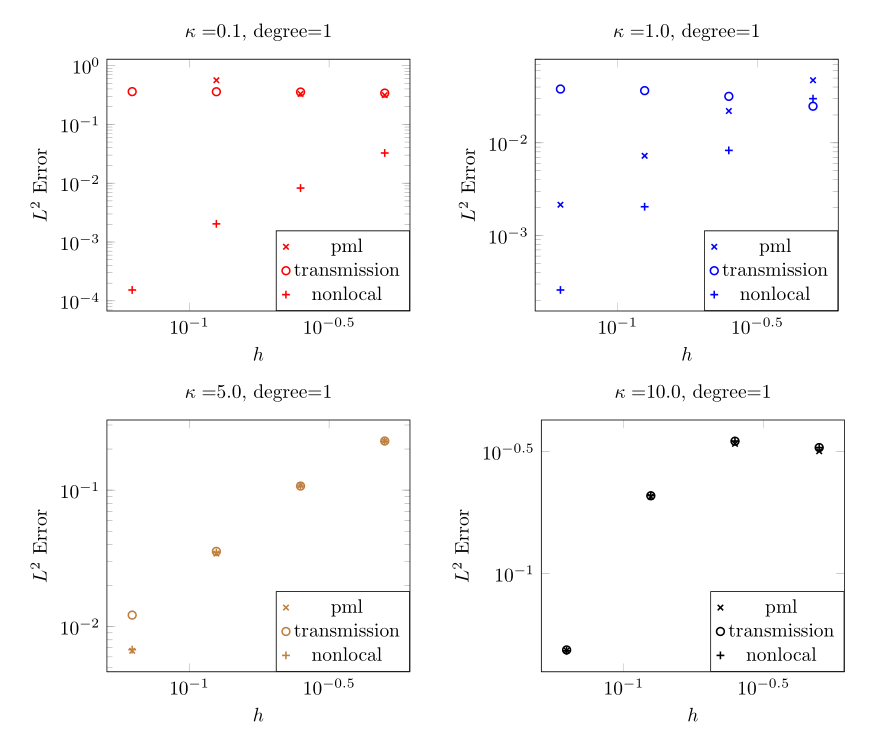
\includegraphics[width=0.8\textwidth]{images/3d-accuracy.png}
    \end{center}
    \end{figure}
\end{frame}

\end{document}
